\part[SCC for LED drivers]{Switched Capacitor Converters for LED drivers}
\label{ch:h_scc}

\chapter{}
Switched Capacitor Converters (SCCs) are \emph{dc-dc} power circuits composed only by switches and capacitors that provide efficient voltage conversion. SCCs have been long known and utilized, initially for voltage multiplication and more recently for voltage regulation as well. Compared to inductor based power converters, the absence of magnetic elements makes them suitable for high density power systems and integrated solutions, such as Power-System-in-Package (PSiP) or Power-System-on-Chip (PSoC). 

The power conversion capabilities and the favorable characteristics for integration combined with the growing necessities for integration in the LED driver circuits was the initial motivation of the presented work. This first chapter will make the reader to understand the operation of the converter, the context of the general applications of SCC and the specific work done related to LED driving.

\section{Operation of Switched Capacitor Converters}

A Switched Capacitor Converter is a electronic circuit only composed by interconnected capacitors and switches that produces voltage-to-voltage conversion. The converter has two o more configuration modes, referred as phases, that sequentially change in order to achieve power conversion. 

\begin{figure}[!h]

\centering
\ctikzset { bipoles/length=1cm}
%\ctikzset { scale=0.5}
    \begin{subfigure}[t]{\textwidth}
    %\floatbox[{\capbeside\thisfloatsetup{capbesideposition={left,top},capbesidewidth=1cm}}]{figure}[\FBwidth]
%{\caption{A test figure with its caption side by side}\label{fig:test}}{
    \centering
    %\ctikzset { bipoles/length=1cm}
        \begin{circuitikz}[american voltages,scale=0.6]
        %\draw (0,11) node[anchor=north]{ };
        \draw
                %Input Supply
                (0,0)  to[V=$v_{i}$]
                %Draw Switches
                (0,10)  --
                (5,10)  to[switch=$s_1$] %S1
                (5,8)   to[switch=$s_2$] %S2
                (5,6)   to[switch=$s_3$] %S3
                (5,4) --
                %left branch
                (3,4)   to[switch=$s_5$]
                (3,2)   to[switch=$s_4$]
                (3,0);

        \draw   %right branch
                (5,4) --
                (7,4)   to[switch=$s_6$]
                (7,2)   to[switch=$s_7$]
                (7,0) -- (0,0);

        \draw %Capacitor C1
               (3,2) -- (2,2) -- (2,4)
                to[pC=$c_1$] (2,8) --
               (5,8);



        \draw %Capacitor C2
                (7,2) -- (8.25,2) --
               (8.25,4) to[pC=$c_2$](8.25,6) --
               (5,6);

        \draw %Capacitor C3
               (5,0) to[pC=$c_3$]
               (5,4);
               
         \draw (7,4) to[short,-o] (10,4) node[anchor=west] {$v_o$};
         \draw (7,0) to[short,-o] (10,0) node[anchor=west] {};
         \draw (10,4) to[open,v^=$v_{out}$] (10,0);

         \end{circuitikz}
     \subcaption{Circuit diagram the two phase 3:1 Dickson Converter.}
     \label{fig:demo_full_sch}
    \end{subfigure}

    \begin{subfigure}[t]{\textwidth}
    \centering
    %\ctikzset { bipoles/length=1cm}
        \begin{circuitikz}[american voltages,scale=0.6]
        \draw (-1,7) node[anchor=north]{ };
        \draw
                %Input Supply
                (-1,0)  to[V=$v_{i}$]
                %Draw Switches
                (-1,6)  --
                (4,6);
                
        %Capacitor C1
        \draw   (4,3) to[pC=$c_1$] (4,6);
        
        %Capacitor C2
        \draw (2,0)to[pC=$c_2$](2,3) --(4,3);
        
        %Capacitor C3
        \draw  (-1,0)--
               (6,0) to[pC=$c_3$]
               (6,3) -- (4,3);

         \draw (6,3) to[short,-o] (7.5,3) node[anchor=west] {$v_o$};
         \draw (6,0) to[short,-o] (7.5,0) node[anchor=west] {};
         \draw (7.5,3) to[open,v^=$v_{out}$] (7.5,0);
         \end{circuitikz}
     \subcaption{First phase, odd switched are closed and even switches are open.}
     \label{fig:demo_full_p1}
     \end{subfigure}

     \begin{subfigure}[t]{\textwidth}
      \centering
      \begin{circuitikz}[american voltages,scale=0.6]
        \draw (0,7) node[anchor=north]{ };
        \draw   %Input Supply
                (-1,0)  to[V=$v_{i}$]
                %Draw Switches
                (-1,6);

        \draw   (5,3) to[pC=$c_2$] (5,6);

        \draw %Capacitor C1
               (2,0)to[pC=$c_1$](2,6) --(5,6);

        \draw %Capacitor C3
               (5,0) to[pC=$c_3$]
               (5,3) -- (5,3);

         \draw (5,3) to[short,-o] (7.5,3) node[anchor=west] {$v_o$};
         \draw (-1,0) to[short,-o] (7.5,0) node[anchor=west] {};
         \draw (7.5,3) to[open,v^=$v_{out}$] (7.5,0);
         
         %\draw ()
         \end{circuitikz}
     \subcaption{Second phase, even switched are closed and odd switches are open.}
     \label{fig:emo_full_p2}
     \end{subfigure}
\caption{}
\label{fig:emo_full}
\end{figure}


\section[Chronological Vision of SCC]{A chronological vision of Switched Capacitor Converters}

The first Switched Capacitor Circuit was proposed in 1919 by Heinrich Greinacher. The \emph{Voltage Multiplier Rectifier}
multiplied the peak voltage of an AC supply to a DC voltage proportional to the number of stages. In 1932 J.D. Cockcroft and E.T.S. Walton used this circuit to generate very high voltage potentials,up to 800 kilovolts, for their particle accelerator ~\cite{30Cockcroft}; the picture of Figure~\ref{fig:Cockcroft_VMR} shows one of the used voltage multipliers. Subsequently, this circuit become widely used in television sets to supply high voltage to the cathode ray tube ~\cite{70Buechel} and later it was used in space applications~\cite{86Weinberg}. D.L. Waidelich and J.S. Brugler made some contributions to determine equivalent series resistance~\cite{44Waidelich,71Brugler} and Brugler and L. Chua proposed a unified approach to generate and analyse new topologies
~\cite{71Brugler,77Lin}.

\begin{figure}[!h]
\centering
 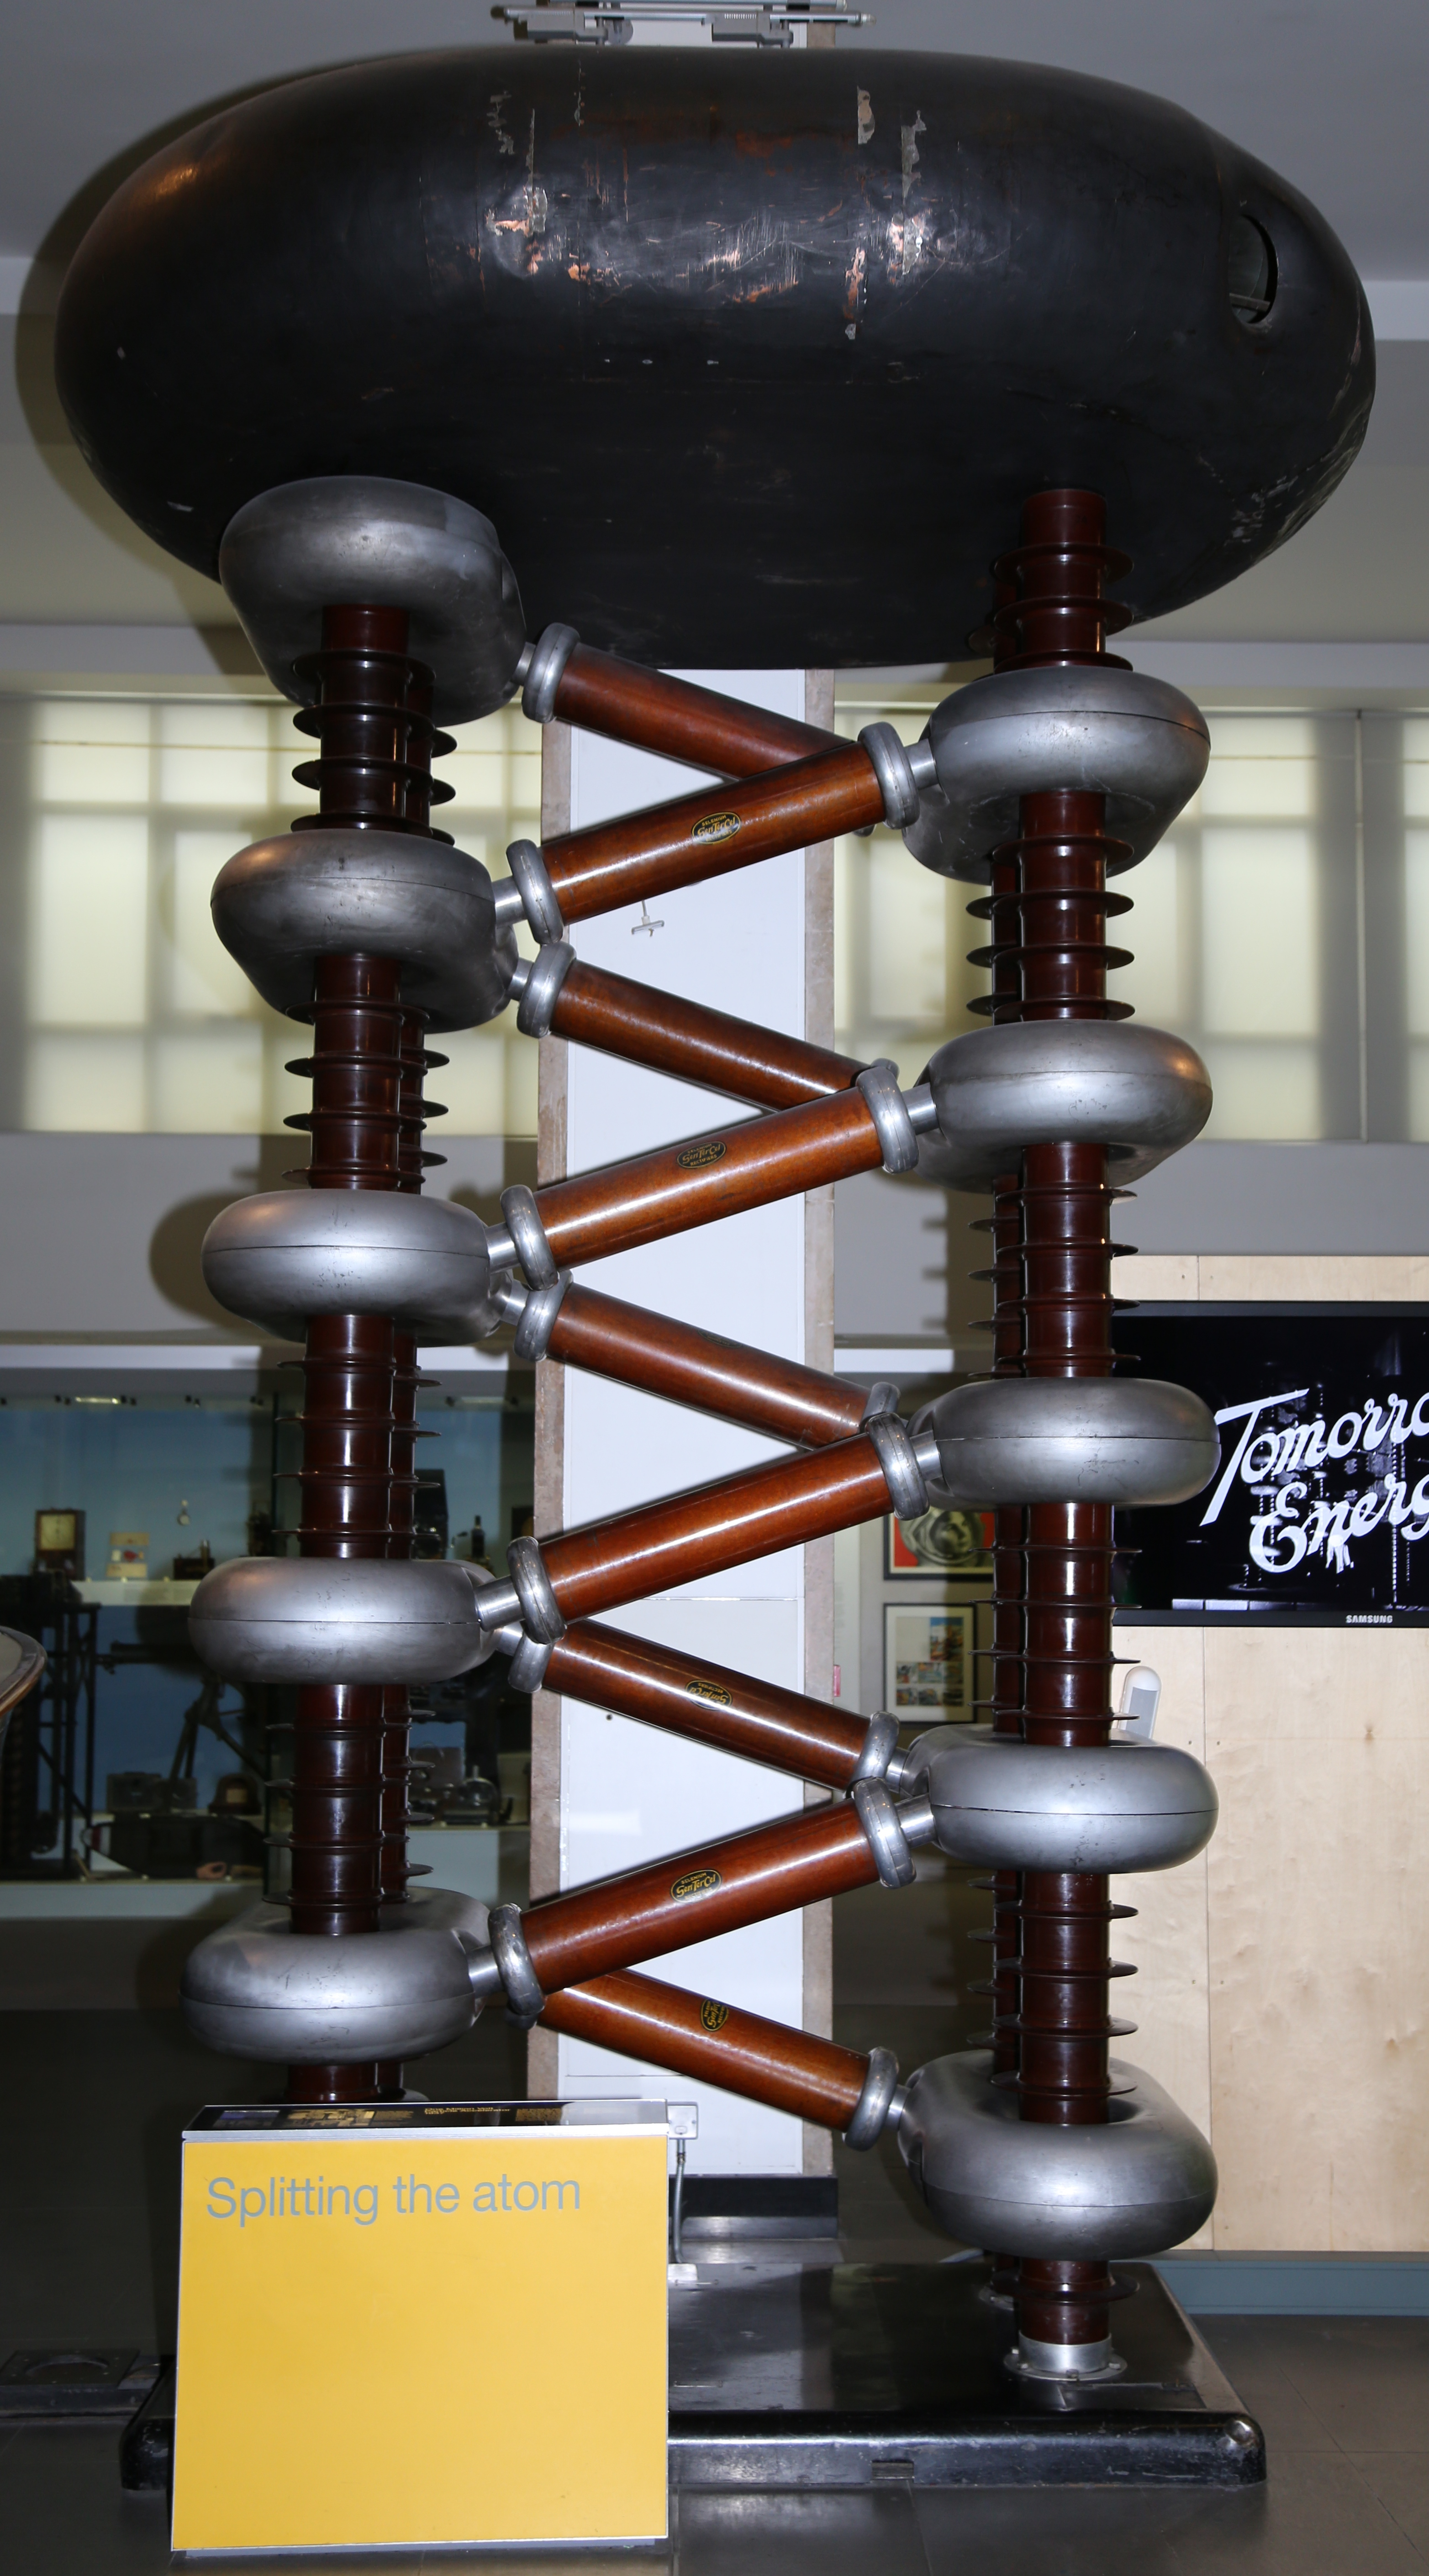
\includegraphics[width=6cm]{./1_modeling/img/CockcroftWaltonGenerator.jpg}
%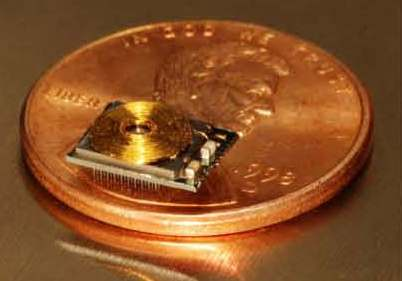
\includegraphics[width=6cm]{./0_intro/img/FSolzbacher01.jpg}
\caption{Cockcroft-Walton voltage multiplier built in 1937 by \emph{Philips Research Labs} in Eindhoven, now exposed in the \emph{Natural Science Museum} of London\\
\emph{Source:"Cockcroft–Walton generator 2012" by Geni. Licensed under GFDL via Wikimedia Commons  %http://commons.wikimedia.org/wiki/File:Cockcroft%E2%80%93Walton_generator_2012.JPG#/media/File:Cockcroft%E2%80%93Walton_generator_2012.JPG
}}
\label{fig:Cockcroft_VMR}
\end{figure}


In 1976, J.F. Dickson ~\cite{76Dickson} introduced a modification of the Cockcroft-Walton circuit to enable the integration of a voltage multiplier in an MNOS non volatile memory IC. The so-called Dickson charge-pump boosted the DC supply voltage proportionally to the number of stages in the pump. At same time, the new circuit mitigated the effects of the integrated capacitor stray capacitances on the voltage gain and reduced the output impedance of the converter increasing the current throughput. After the Dickson charge-pump other topologies~\cite{09Seeman} have been reported, such as the series-parallel converter ~\cite{94Ngo,94Cheong}, which allowed rational conversion ratios. F. Ueno \textit{et al.} ~\cite{91Ueno} presented yet another topology with conversion ratios corresponding to Fibonacci series,$k=1,2,3,5,8,..$ ,achieving higher conversion ratios using fewer capacitors ~\cite{95Makowski,09Allasasmeh}.  F.L. Luo  ~\cite{02Luo} proposed a topology cascading voltage doublers cells where the conversion ratio follows a quadratic relationship with the number of cells, and J. A. Starzyk ~\cite{01Starzyk} reviewed the same concept with a multi-phase topology that can achieve the same gain with fewer capacitors.



Two important concepts have been introduced to SC converters in order to reduce the current ripples and conduced Electromagnetic Interferences (EMI):
\begin{description}
  \item[Interleaving] also improves the efficiency since the it can reduce the value for the output capacitor. There are different reported implementations of 2-phase ~\cite{07Chang,99Chung}, 16-phase ~\cite{09Breussegem,14Andersen}, 32-phase~\cite{10Le} 64-phase~\cite{15Andersen}.
  \item[Current Mode] Charge-Pumps ~\cite{96Zhu,09Das} where the process of charge or discharge -or both- are controlled with a current source.
\end{description}

There are other innovative approaches where SCCs are combined with inductor based converters, also referred as \emph{hybrid} SCCs. The combination of both achieve large conversion ratios with tighter regulation. There are a large number of hybrid solutions where a SC cell is integrated into an inductor based converter ~\cite{05Axelrod,08Axelrod, 11Mayo,11Miranda,12Kline}. Lately, a couple of papers ~\cite{12Zhigang,11Dazhong} presented a Maximum Power Point Tracking (MPPT) converter for Photovoltaic (PV) cells employing a SC converter in parallel with an inductor based converter. This hybrid combinations offer another family of converters known as \emph{Resonant Switched Capacitor Converters} (RSCC), where the capacitors are charged through resonant transitions, thus eliminating the capacitor charge transfer losses.  K.W.E. Cheng ~\cite{01Cheng} in 2001 presented an early  work where in the topic using inductors limit the currents thought the capacitors and charging and discharging the capacitors with resonant transitions.  Subsequently, many publications appeared ~\cite{05Lee,10Cao,11Gebben,07Shoyama} presenting applications and uses of this converter family. Initial RSCC topologies made use of multiple inductors to guarantee a resonant transition for all capacitors, recent works~\cite{13Kesarwani,13Schaef,14Kesarwani,15Schaef} presented new topologies that reduced the number of inductors to achieve these resonant transitions.


\section{Sate of the Art of Switched Capacitor LED drivers}

One of the most popular application of SCCs is indeed as LED drivers for portable devices. Low power White LEDs (W-LEDs) are widely applied for back-lighting Liquid Crystal Display (LCD) in devices such as laptops, mobile phones and tablets. These applications require to generate a voltage above the LED forward voltage ($v_f$) from the battery, what can not been achieved with just using a linear drivers since the battery voltage is easily below to $v_f$  as it discharges. Normally theses drivers implement step-up or step-down to convert the battery right above the $v_f$.

\begin{figure}[t]
    \centering
    \begin{circuitikz} [scale=0.65]
    \ctikzset{bipoles/length=0.85cm}
   \draw[thick] (2.5,0.25) --
                (2.5,6.5) --
                (11.5,6.5) --
                (11.5,0.25) --
                (2.5,0.25);

    %Draw SCC block with capacitors
    \draw (3,1) --
          (3,6) --
          (5,6) --
          (5,1) --
          (3,1);

    \draw (4,1.25) node[rotate=90,anchor=west] {\emph{Multi-ratio SCC}};

    \draw (3,2) --
          (1.5,2) to[capacitor]
          (1.5,3) --
          (3,3);

    \draw (3,4) --
          (1.5,4) to[capacitor]
          (1.5,5) --
          (3,5);

    \draw (5,5.5) to[short,-o] (14,5.5);
    \draw (13,5.5) to[capacitor] (13,4.5) node[sground]{};

    \draw (4,1) -- (4,0) node[sground,scale=0.75]{};

   %Draw linear drivers
   \draw  (4,0.5) -- (10.5,0.5) -- (10.5,1);

   %First transitor
   \draw   (10,1) -- (10,1.5) node[npn,anchor=E,scale=0.5](npn1){}
           (npn1.C) -- (10,2.75) to[short,-o] (12,2.75);

   %Second transitor
   \draw  (10,1) -- (11,1)
           node[npn,anchor=E,scale=0.5](npn2){}
           (npn2.C) -- (11,2.25) to[short,-o] (12,2.25);

   %Controller box
   \draw (5.5,1) -- (8.5,1) -- (8.5,3) -- (5.5,3) -- (5.5,1);
   \draw (5.75,2) node[anchor=west, text width = 1.75cm]{Intensity Controller};
   \draw (npn2.B) -| (8.5,2);
   \draw (npn1.B) -| (8.5,2);

   %LEDs

   \draw [dashed] (14.25,5.5) to[short,o-] (15,5.5)
                    to[leD*] (15,2.75) to[short,-o] (12.25,2.75);

   \draw [dashed] (15,5.5) -- (17,5.5)
                    to[leD*] (17,2.25) to[short,-o] (12.25,2.25);

   %Add battery

   \draw (-1,0) node[sground,scale=0.75]{};
   \draw (-1,0) to[battery] (-1,6)
         -- (2.5,6);

    \end{circuitikz}
    \caption{Block diagram of a generic driver for backlighting applications.}
    \label{fig:backlight_LED}
\end{figure}

There is a large portfolio of available ICs, designated as Charge-Pumps (CPs), for driving LEDs in portable devices. Some commercial products are for instance  the \emph{MAX88779} \footnote{Maxim\textsuperscript{\textregistered} Charge Pump for Backlight/Flash/RGB LEDs with Safety Timer } or the \emph{MCP1252/3} \footnote{Microchip\textsuperscript{\textregistered} Low noise, Positive-Regulated Charge Pump}. These circuits  can drive withe, RGB or Flash LEDs from a Lithium-Ion battery only by adding a few external capacitors capacitors.  Generally these chips integrate an multi-target SCC with different conversion ratios (1:1, 3:2, 2:1) along with a series current regulator for each LED channel a shown in the block diagram of Figure~\ref{fig:backlight_LED}. Various publications ~\cite{07Feng,09Wu,10Yin} proposed enhancements in the architectures in order to reduce the parasitic losses bringing the efficiency close to the theoretical limit. Such drivers are used in applications below a 1$W$ and currents below hundred $mA$, their efficiency derates as the LED voltage moves away from the target voltage.

Besides the backlighting ICs, there are no other commercial LED drivers based on SCC. However that topic has been present in several research publications for the last years with few interesting publications targeting mains connected drivers. In 2008, K.H. Lee \emph{et al.}~\cite{08Lee} presented a SC step-down converter composed of several cascaded Series-Parallel that supplied from rectified 220$V_{rms}$ an LED string of 75V at 15W. In the proposed solution the LEDs are directly supplied using flying capacitors what produces pulsating currents in the string and its average values is controlled modulating the frequency of the converter. The cascaded topology minimized the number of components, switched and capacitors, for the required conversion ration (fixed by the LED string).

In 2012, M. Kline \emph{et al.} ~\cite{12Kline} proposed a isolated \emph{DC}/\emph{DC} converter that combined a SCC stage with series-LC resonant converter.  The SCC stage decreased  the rectified mains voltage, reducing the voltage stress in switches, capacitors and the elements of the resonant tank. The lower voltage stress allows a reduction in the volume of the passive components and the total area in the silicone. By controlling the frequency and the duty cycle of the SCC stage current through the LEDs can be regulated, resulting in a very efficient solution. In a recent publication they presented an implementation where power train and control where integrated in different stackable ICs modules~\cite{13Kline}.

The different applications show an increasing interest in using SCC for LED drivers. It is evident that the approach used in portable devices can no be further extended in for high powers and higher voltages. The use of a bear SCC can never satisfy the requirements of LED drivers due to the following facts:
\begin{itemize}
  \item Only provide voltage-to-voltage conversion
  \item Fixed conversion ratios
  \item Regulation is provided by series shunting
\end{itemize}
These limitations combined with the abrupt characteristics I-V of the LEDs makes barely impossible to provide high efficient solutions with the single use of SCC. The converters would require to have a large number of conversion ratios with a very large granularity to avoid uncontrolled currents flowing through the LEDs.

The research presented in this work aims to explore the possibilities of the SCC for LED drivers and the conducting path is based in the combination of the with inductors. The overall solution improves the power density and reduced form factor of the present solutions.



\section*{Power Levels and Integration}

There are not intrinsic implications that limit the output power of a Switched Capacitor converter, but the boundary conditions. There are implementations ranging from tens of milliwatts to tens of kilowatts, where the difference only relies in the used technology. They can be classified in 3 groups: Fully integrated circuits, integrated circuits with external capacitors and discrete solutions.

Full integrated converter are suitable for very lower power applications from some microwatts up to some tens of milliwatts. These solutions are implemented in standard processes (CMOS, BiCMOS or Bipolar) where the priority is in achieve an integrated solution rather than efficient. These converters have very poor efficiency up to 60\%, due to the low energy density and poor quality of the capacitors available in those processes. The second group overcomes this problem using external capacitors. These converters integrate the control and the power train in a single chip with a stadard CMOS process, offering  output power up to one watt and peak efficiencies of 95\%. In this case, the CMOS switches limit the converter efficiency and scalavility in power.
The implementations with discrete components enable output powers up to kilowatts with peak efficiencies above 95\%. Discrete semiconductor switches can offer lower channel resitance and better switching characterisitcs, reducing ohmic resitance and enabeling higher switching frequencies.  \emph{ \color{red} Silicon power MOSFET are the dominant in discrete implementations, but recent publications used Galiun-Nitride HEMT switches ~\cite{11Scott,12Scott}}.

The limiting factor of the output power of a SC converter is driven by the boundary conditions of the technology. Up to now, integrated SC converters designs have been covered addressing the problem with the standard process in VLSI, in order to have compact power conversion units at the lowest cost. The current technologies can easily improve the present solutions, for instance, a Power-System on Package (PSoC) integrating switches and capacitors would already reduce the series resistance of the pins and optimize the silicon die area of the present integrated converters with external capacitors. The current technologies offer the possibility to achieve integrated SC converters processing higher powers, but it would require to combine them in non-standard processes.

\emph{\color{red} Missing refs!}


%\bibliographystyle{plainnat}
%\bibliography{phd_bib} 